\chapter{Examples and Snippets}\label{cha:A}

\section{Pseudocode}

\begin{algorithm}
\begin{algorithmic}[1]
\caption{Flow-Cut Algorithm}\label{algo:flowCut}
\Procedure{Flow-Cut}{P}\Comment{This part is not essential.}
\State $cg \gets$ \Call{deriveCausalGraph}{P}
\State $\langle$l,c,r$\rangle \gets$ \Call{makeInitialCut}{cg}\Comment{3-tuple of
sub-graphs,$\langle left,cut,right\rangle$}
\State $minimal \gets false$
\While{not $minimal$}
\State $minimal \gets$ \Call{shrinkCut}{$\langle$l,c,r$\rangle$}\Comment{Hill
climbing algorithm}
\EndWhile
\State \Return \Call{createSolveProblems}{subset,l,r,P}
\EndProcedure
\end{algorithmic}
\end{algorithm}

\begin{algorithm}
\begin{algorithmic}[1]
\caption{DXBB algorithm in planning}\label{algo:genericSearch}
\Statex \textbf{Input}: Planning task $\Pi$ and heuristic $h$
\Statex \textbf{Output}: A least-cost path from $s_0$ to $s_G$
\State $Open_F = s_0$, $Open_B = s_G$
\State $Closed_F = \{\}$, $Closed_B = \{\}$
\While{\textsc{StoppingCondition} not fulfilled}
\State $Dir,\ State =$ \textsc{Choose}$(Open_F,Open_B,h)$ 
\Comment{$Dir$ can assume $F$ or $B$.}
\State Add $State$ to $Closed_{Dir}$
\State $Successors = expand_{Dir}(State)$
\State Add $Successors$ to $Open_{Dir}$
\EndWhile
\State \Return \textsc{Solution}
\end{algorithmic}
\end{algorithm}

\newpage
\section{Formulas}

\begin{equation}
\begin{aligned}
0(\langle left,cut,right\rangle) &= 2^C * 2^{|left|+|cut|} + 2^C * 2^{|right|+|cut|}\\
&= 2^{C+|left|+|cut|} + 2^{C+|right|+|cut|},
\end{aligned}
\end{equation}

\begin{align*}
pr_F(u) &= \max(g_F(u)+h_F(u), g_F(u)/p),\\
pr_B(u) &= \max(g_B(u)+h_B(u), g_B(u)/(1-p)),
\end{align*}

\section{Figures}

\begin{figure}[ht] % use H for forcing the position
    \centering    
    \begin{minipage}{.49\textwidth}
        \centering
        \resizebox{0.8\textwidth}{!}{%
        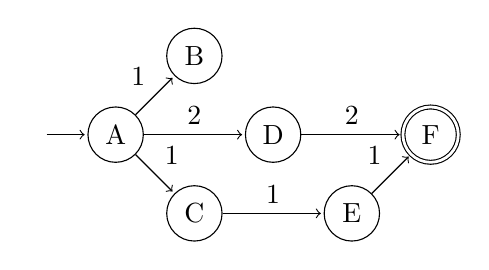
\begin{tikzpicture}[shorten >=1pt, auto, node distance=3cm,
   base_node_style/.style={draw, inner sep=0.5pt, outer sep=0.2pt, draw=black, text=black},
   node_style/.style={base_node_style, circle, minimum size=20pt},
   edge_style/.style={->,draw=black},
   goal_style/.style={node_style,double, double distance=1.0pt}]
   
    \node[] (s) at (-1,0) {};
    \node[node_style] (A) at (0,0) {A};
    \node[node_style] (B) at (1,1) {B};
    \node[node_style] (C) at (1,-1) {C};
    \node[node_style] (D) at (2,0) {D};
    \node[node_style] (E) at (3,-1) {E};
    \node[goal_style] (F) at (4,0) {F};

    \path [edge_style, ->](s) edge (A);
    \path [edge_style](A) edge node {$1$} (B);
    \path [edge_style](A) edge node {$1$} (C);
    \path [edge_style](A) edge node {$2$} (D);
    \path [edge_style](D) edge node {$2$} (F);
    \path [edge_style](C) edge node {$1$} (E);
    \path [edge_style](E) edge node {$1$} (F);
\end{tikzpicture}





        }
    \end{minipage}        
    \begin{minipage}{.49\textwidth}
        \centering
        \includegraphics[width=0.9\linewidth]{graph}
    \end{minipage} 
    \caption{(Left) A tikz figure included from another file. (Right) An important graphic.}
    \label{fig:gmx2}
\end{figure}

\section{Tables}\label{sec:A:tables}
\begin{table}[H]\centering\ra{1.3}
\begin{tabular}{c|c|cccc}
\midrule
\multicolumn{1}{c}{\textit{Blocks}} &  &\multicolumn{4}{c}{\textit{Expansions (\#)}}\\
\cmidrule(){3-6}
 & \textit{Algo} & $h^0$ & $h^{max}$ & $h^m$ & $h^{lmcut}$\\
\toprule
\multirow{ 2}{*}{p4-0}& $A^*$ & 85 & 21 & 8 & 7\\
& \texttt{NBS} & 19 & 10 & 10 & 9 \\
\midrule
\multirow{ 2}{*}{p4-1}& $A^*$ & 58 & 21 & 12 & 12\\
& \texttt{NBS} & 22 & 13 & 13 & 13\\
\midrule
\multirow{ 2}{*}{p4-2}& $A^*$ & 52 & 15 & 7 & 8\\
& \texttt{NBS} & 19 & 10 & 8 & 7\\
\midrule
\multirow{ 2}{*}{p5-0}& $A^*$ & 467 & 147 & 32 & 21\\
& \texttt{NBS} & 43 & 35 & 24 & 21\\
\bottomrule
\end{tabular}
\caption{A beautiful table with multirow, multicolumn, toprule, midrule, and bottomrule.}\label{tab:A:tables:sampleTable}
\end{table}


\newpage
\section{Definition and Background}

\begin{quotation}
"Planning is the reasoning side of acting. It is an abstract, explicit
deliberation process that chooses and organizes actions by anticipating their
expected outcomes." ~\citep{ghallab2004}
\end{quotation}

Classical planning is about determining the course of action which leads to the best possible outcome. The used framework consists of three different parts: the input, the algorithm, and the output. A \emph{problem instance} functions as the input and is described by the corresponding \emph{planning task}. A \emph{planning algorithm} solves the problem instance and computes the solution \emph{plan} as output. 

\begin{bgDef}[Planning Task]
We are using an adaptation of the finite domain $SAS^+$ formalism introduced by \cite{backstrom1995complexity} to describe a planning task formally. A planning task is a 4-tuple $\Pi = \langle \mathcal{V},\mathcal{A},\mathcal{I},\mathcal{G} \rangle$, where 
\begin{itemize}
    \item $\mathcal{V}$ is a finite set of \emph{state variables}, each $v \in \mathcal{V}$ has an associated finite domain $D(v)$, which specifies valid variable assignments.
    \item A \emph{partial state} $\hat{s}$ is a mapping of state variables $v \in \mathcal{V}$ to a value consistent with their defined domain. These assignments are written as $s[v] \in D(v)$. $var(s) \in \mathcal{V}$ is a finite set which lists all variables that have an assignment in the specified partial state. 
    \item A partial state $s$ is called a \emph{state}, if all variables $v \in \mathcal{V}$ have a valid assignment given by $s$, hence $var(s)=\mathcal{V}$.
    \item $\mathcal{A}$ is a finite set of actions, each $a \in \mathcal{A}$ is a triple $(\pre(a),\eff(a),cost(a))$, where
    \begin{itemize}
        \item $\pre(a)$ is a partial state defining the \emph{preconditions}.
        \item $\eff(a)$ is a partial state defining the \emph{effects}.
        \item $cost(a) \in \mathbb{R}_0^+$ is the associated \emph{cost}.
    \end{itemize}
    \item $\mathcal{I}$ is a state defining the \emph{initial state}.
    \item $\mathcal{G}$ is a partial state defining the \emph{goal} conditions.
\end{itemize}
\end{bgDef}

A partial state $\hat{s}_1$ is a subset of another partial state $\hat{s}_2$ when $\hat{s}_1[v] = \hat{s}_2[v]$ for all $v \in var(\hat{s}_1)$ holds and is written as $\hat{s}_1 \subseteq \hat{s}_2$. A partial state \emph{complies} with another partial state if one is a subset of the other. Action $a$ is \emph{applicable} in state $s$ under the condition that $\pre(a) \subseteq s$. Applying action $a$ on state $s$ is denoted by $s\apply{a}$ and modifies the state $s$ to comply with the partial state $\eff(a)$. In classical planning we search for a sequence of actions, which when applied on the initial state $\mathcal{I}$ yield a resulting state $s$ where $\mathcal{G} \subseteq s$ holds. Such a sequence is called a \emph{plan}: $\pi = (a^1,a^2,\dots,a^n)$. The cost of a plan $\pi$ is given by the summed cost of all included actions: $cost(\pi) = \sum\nolimits_{i=1}^{n}cost(a^i)$. If no plan exists then the planning task is \emph{unsolvable}, otherwise, there are plans and thus at least one of those plans has the minimal cost compared to the others and is called the \emph{optimal plan}. A commonly used method to determine the optimal plan from a planning task, is to first build the implicitly defined \emph{transition system} and then find the plan by \emph{heuristic search}.


\section{Labelling Convention}

The first part of a label denotes the type of caption it belongs to: \emph{cha}, \emph{sec}, \emph{par}, \emph{fig}, \emph{tab}, or \emph{algo}. Followed by the hierarchy of its position and a name representing it. The labels should be all lowercase, expect for the Appendices A and B, as well as any camel case used when necessary. The following list shows the labels used for the thesis structure:

\begin{itemize}
  \item Introduction - cha:intro
  \item Background - cha:bg
  \item (Related Work - cha:rw)
  \item Main Part - cha:main
  \item Experiments - cha:exp
    \begin{itemize}
      \item sec:exp:exp1
      \item sec:exp:exp1:setup
      \item sec:exp:exp1:results
      \item par:exp:exp1:results:typeA
    \end{itemize}
  \item Conclusion - cha:conclusion
  \item Appendix A - cha:A
  \item Appendix B - cha:A
\end{itemize}


